\chapter{Background}

While the Earth's atmosphere is thick enough to cause more objects that pass through it, some can and will make it through. Theses are the objects of most importance to those observing fireballs, meteoroids, and meteors. This chapter will provide a more in-depth look at what classifies an object as a fireball, how these fireballs are detected both by other systems around the world and the D6, and discuss why and how the detected images are analyzed.

\section{What Exactly are Fireballs?}

The first thing to take into account when discussing meteoroids, meteors, fireballs, and even asteroids, is that they are all different and shouldn't be used interchangeably. 
An asteroid is not a meteoroid, a meteoroid is not a meteor, a fireball is a classification of meteor, and a bolide is a fireball that blows up in the atmosphere. 
This section will go into a little more detail regarding the various definitions of these space objects, 

Asteroids are meteoroids that are greater than 1 meter wide, as can be seen in figure 3, they tend to be concentrated outside of the Earth's orbit, as can be seen in the third figure.
As can be seen from this concentration, and from what has been determined by the scientific community, large asteroid impacts tend to occur rather rarely, with "an automobile sized asteroid" entering the atmosphere about once a year \cite{atkinson_2018}. 
Meteoroids however, are the little siblings of asteroids, and are of just as much interest.

\begin{figure}
    \centering
    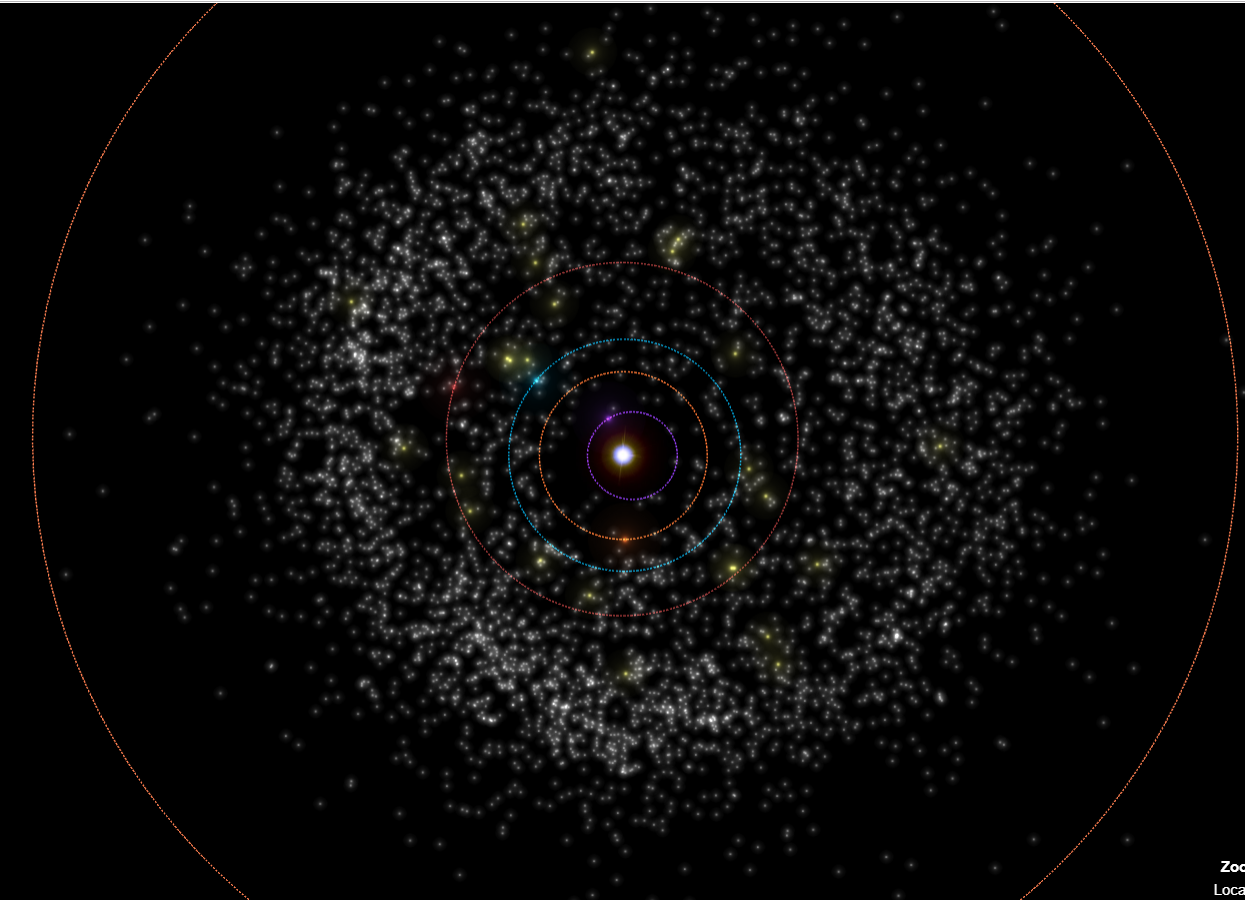
\includegraphics[width=12cm]{Solar-System-Asteroids.png}
    \centering
    \caption{Image of asteroid plots in our Solar System, courtesy of Asterank, as can be seen the asteroids mainly orbit outside the orbit of the Earth, though some do merge in and out of the Earth's orbit.}
    \label{Figure 3}
\end{figure}

Meteoroids are any bits and bobs of cosmic space debris that are up to 1 meter in width, from dust to small pieces of rock blasted off from asteroid collisions. 
The only true difference between an asteroid and a meteoroid is that one is large, while one is usually much smaller, with the meteroid being frequently only millimeters in size \cite{atkinson_2018}. 
When both asteroids and meteoroids hit the atmosphere and begin leaving a streak of fire across the sky, they are then referred to as meteors. 
While meteors are harmless most of the time, they can turn into bolides, also known as fireballs \cite{atkinson_2018}. 

Fireballs, or bolides, will be the main focus of the project, as they are what are being observed for by the D6 and the other detection systems that the D6 will be compared to when determining it's effectiveness. 
Fireballs are meteors that have especially bright trails, and tend to either burn out in the atmosphere, explode, or leave behind a meteorite like the one that occurred over Spain, Portugal, and France, with a meteorite being left behind in northern Palencia \cite{Villabeto}. 
In the next segment a more in depth look will be taken at the different methods used to detect the fireballs, as well as some of positives and negatives for each of these detection methods.

\section{Methods of Detection}
The main way that fireballs are detected is through the use of a camera of some variety and design.
Although the type of camera and how it's used can vary widely from project to project, as will be seen below.
The other important aspect when detecting fireballs is the way the data is catalogue, stored, and analyzed, with multiple computer stations crunching numbers being the common method employed by most systems.
\subsection{Current Methods of Detecting Fireballs}
One of the major detection networks is called CAMS, or, Cameras for Allsky Meteor Surveillance. 
The goal of this NASA funded project is to validating unconfirmed meteor showers by measuring velocity vectors and times of arrival and from that information, determining if various detected meteoroids and fireballs originated from the same group passing through the Earth's orbit \cite{jenniskens}. 
The stations for the detection network contain a box within which twenty Watec 902 H2 Ultimate video cameras, an interesting feature of this camera setup is that it comes with a sun shade, which can be used to protect the setup from bad weather. 
The sun shade also helps protect the sensitive cameras from direct sunlight during daytime hours \cite{jenniskens}. 
An important feature of this setup to note is that the camera also has a battery mounted nearby to support it, as well as the linux surveillance servers required to process and store the data from each of the cameras.
As can be seen in Figures 4 and 5, the total setup is fairly bulky, although the use of an array of cameras for comparison will allow for fairly good detail in any capture images, as well as the capability to determine the velocity of a fireball as it moves across the array.

\begin{figure}
    \centering
    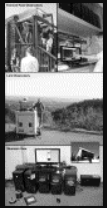
\includegraphics[scale=1.5]{CAMS-Server-Setup.png}
    \caption{Image of the Server setup for the CAMS fireball detection network. This image is taken from \cite{jenniskens} so that readers can have a good idea of how bulky the conventional support systems can be.}
    \label{Figure 4}
\end{figure}

\begin{figure}
    \centering
    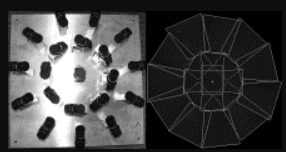
\includegraphics[scale=1.5]{CAMS-Camera-Setup.png}
    \caption{Image of the Camera setup for the CAMS fireball detection network. This image is taken from \cite{jenniskens} so that readers can also have a good idea of how bulky the camera setups for conventional detection systems can be.}
    \label{Figure 5}
\end{figure}

Another system is the SPMN, or Spanish Meteor Network, where instead of having an array of cameras at each station, each video station uses a high sensitivity CCTV camera, with there being 11 of the high sensitivity cameras in total \cite{SPMN}. 
An interesting feature of this system is that each camera will have an Aspherical fast lens that will have a focal length ranging from 2.6 mm, which is a fish-eye lens, to 12mm and a focal ratio between 1.2 and 0.8 for the imaging reflective lens. 
These different lens types will allow various areas of the sky to be covered by each and every camera, and images across the entire field of view can be captured \cite{SPMN}.
As with the CAMS system, the SPMN can also determine the velocity of a fireball or bolide by capturing the meteor and tracking it across the sky using a video time inserter that has a GPS device. 
This allows for an accuracy of $10^-1$ seconds while tracking the meteor along its path across the night sky \cite{SPMN}.

A third system is the Canadian Automated Meteor Observatory, or CAMO for short.
This sytem is rather different from the previous two, with CAMO only consisting of two stations, near Tavistock, Ontario, Canada, and one near Elginfield, Ontario, Canada.
One of the cameras is a wide field setup that detects the meteor at first, helping control two mirrors that reflect the light from the meteor into the narrowfield camera\cite{subasinghe_campbell-brown_2018}.
The two different cameras have other purposes, the capture from the wide-field is used to determine the light curve calculation, which will be discussed in more detail later\cite{subasinghe_campbell-brown_2018}.
The narrow-field camera allows for the fragmentation of the meteor to be analyzed \cite{subasinghe_campbell-brown_2018}.


\subsection{The Willamette University D6 Allsky Camera}

The third detection system that will be discussed in this paper is of course, the Willamette University D6 AllSky Camera. 
The D6 was created in 2016 to, like the previous two detection systems, detect fireballs streaking across the night sky.
The idea behind the D6 is to create a system that is cheaper and easier to move than systems such as CAMS or SPMN. 
To do this, a Raspberry Pie was used as the computational support for the camera system, instead of the more traditional number crunching tools used in CAMS of SPMN \cite{McSwain}.
The D6 itself looks a bit like a short traffic bollard, with a plastic dome covering the Watec902H2 CCD camera, and a PVC pipe acting as the housing for all the internal units of the D6.
Inside, besides the camera and Raspberry Pi, is a thermostat with accompanying heater to ensure that moisture doesn't accumulate inside the housing, as well as a digitizer to convert the film taken by the camera from analog to digital so that it can be analyzed. A image of the camera from PJ Gibsons thesis can be found in figure 6.
Some benefits of this system are that it is in fact very mobile compared to other systems with servers, dedicated power and data cables, and outbuildings to store the servers and any scientists on scene to review the data.
While setup for the systems that support the camera themselves are bulky, as could be seen in previous figures of other systems, the camera setups also tend to be bulky and rather immobile, making it difficult to move if a better location is found.
There are of course, also some downsides to the D6, such as that with only one, it can be difficult to determine the velocity of a fireball, so we have to rely on estimates of the velocity if we want to formulate any true observations from the fireball capture, such as its mass, energy, and flux.
it should be noted that the camera used by the D6 is the same as that used by the CAMS all-sky network, as it was determined to be the best for the task at hand by other parties\cite{jenniskens}.

\begin{figure}
    \centering
    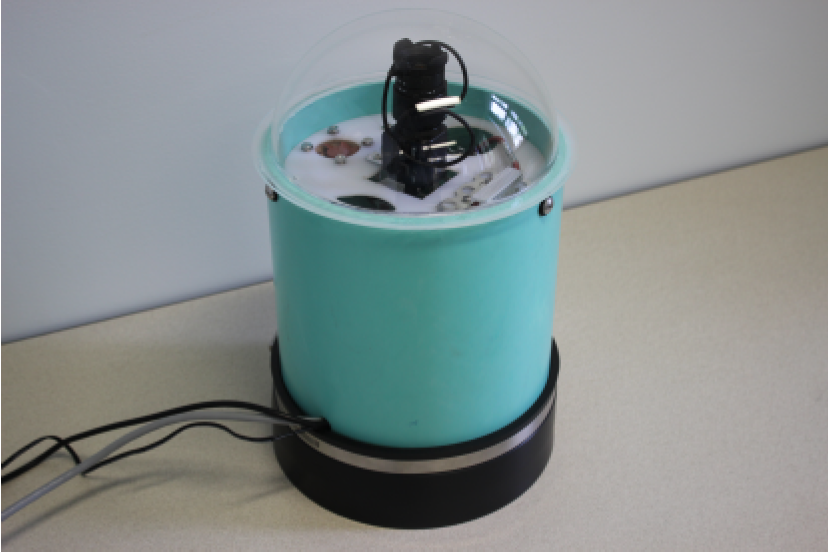
\includegraphics[width=10cm]{D6-Camera.png}
    \caption{This is an image of the Willamette University D6 AllSky Camera setup. As can be seen it's not that large compared to other setups, with both camera and storage systems being in the same compact container. Image taken from PJ Gibson's thesis on the D6 \cite{Gibson}}
    \label{Figure 6}
\end{figure}

When the camera detects a fireball passing through its field of view, it takes footage of said event, and then the footage in converted by the digitizer into a form suitable for the Raspberry Pi to collect and store, with the data being accessed by a laptop at a later date for future analysis using code that will be discussed in the next section.

\section{Previous Work Done on the Project}

\subsection{The Camera Code}
The first step in the camera code is for when the Pi receives an image from the camera, it logs and timestamps the frame, while also checking to make sure that the frames being stored do in fact contain a fireball and not say, a bug or some other random animal flying cross the view-frame\cite{McSwain}.
This system has been refined from the first concept over the years by Doctor Rembold to the point where it is the case that the only frames being stored contain either a fireball or, once in awhile, a bat or some other nocturnal creature.
Currently most other processes that involve analyzing the data take place outside of the camera on a computer that siphons the frames collected by the Raspberry Pi to it's own storage system.

\subsection{Photometry}

The photometry tool that will be used to analyze a fireball is the GUI created by Luke Russell, an image of it can be seen in figure 6\cite{Russell}.

\begin{figure}
    \centering
    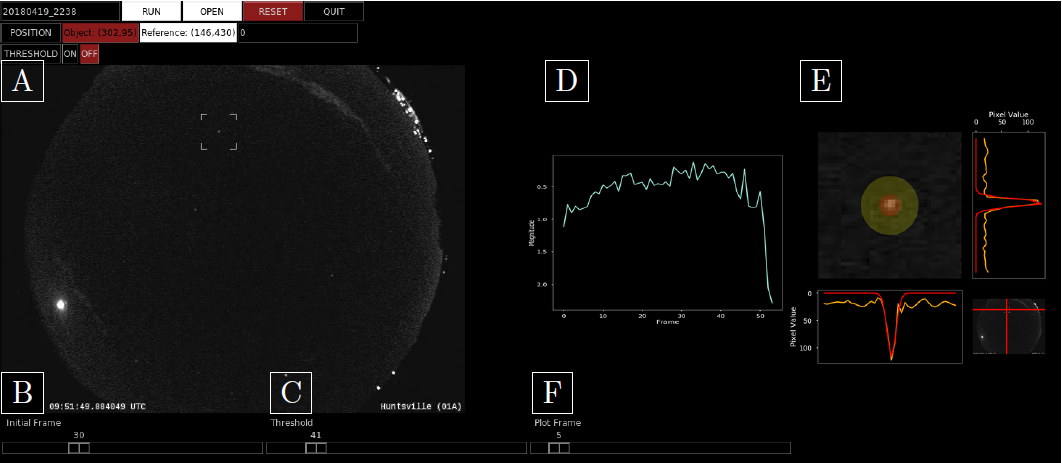
\includegraphics[width=10cm]{Russell-GUI.png}
    \caption{Image of Luke Russells Photometry GUI, this provides an idea of the interface that is used to determine the luminosity of a fireball. This image is taken from his thesis \cite{Russell}}
    \label{Figure 7}
\end{figure}

Some useful equations to keep in mind are 

\begin{equation}
    L = (SA)I
\end{equation}

Where L is the luminosity of the object, I is the intensity of the fireball, and SA is the surface area that the light is spread over. If it is assumed that the light is radiated outward equally in each and every direction, the above equation becomes

\begin{equation}
    L_(obs)=4*pi*r^2*I
\end{equation}

With the intensity being converted to luminosity, the luminosity can be used to find the kinetic energy, with the connection between the two being

\begin{equation}
    L = tT
\end{equation}

With L remaining the luminosity, T being the kinetic energy,  and t being the luminous efficiency, which is the proportion of a fireballs energy dissipated into light. With this equation in mind, we can then switch our focus to determining the mass of the fireball.

First, we begin by manipulating the equation such that 

\begin{equation}
    T = ((v^2)/2)(dm/dt)
\end{equation}

With m, t, and v, being the standard units in physics of m for mass, v for velocity, and t for time.
With the knowledge of the equation for luminosity, we can manipulate it such that
\begin{equation}
    T = L/t
\end{equation}
\begin{equation}
    L/t=((v^2)/2)(dm/dt)
\end{equation}
\begin{equation}
    m=\int \frac{2L}{tv^2}dt
\end{equation}

And thus, by making assumptions around what the velocity of the fireball is, as there is only one camera, the luminosity of the fireball, and the luminous efficiency, along with the length of time the fireball is captured for, the mass of the fireball can be found.
The luminous efficiency of the fireball can be assumed based on Peter Browns fit of a plot, with t being\cite{PBrown2002}:

\begin{equation}
    t = (0.1212\pm 0.0043)(E_o)^{0.115\pm 0.075}
\end{equation}

Where $E_o$ is the optical energy.

\subsection{The Observational Area}

Unfortunately, it is rare to have a perfectly cloudless night in salem Oregon, what with wintery weather being a fact of life around 8-9 months of the year, with only really the summer to have dependable clear skies.
Therefore, it becomes important to determine the surface area that the camera is capturing, as with that info in hand, it becomes possible to also determine the luminosity of a fireball.
This is done by first collecting images of the sky before and following a fireball event, these images are first run through a threshold, so that the image will go from a grayscale to purely black or white, with the white being the clouds and the black being the sky, this image is then reversed and tweaked and compared to a sky coverage map, we can determine the areas occupied by clouds\cite{Gibson}. 
With this "multiplied" by the fireball capture image so that the clouds in the capture image are essentially deleted from the picture, thus giving a capture that can then be examined to determine the luminosity of the fireball, and from there any other pieces of information that might be of interest.
An example of this thresholding and manipulating process for images can be seen in figure 8, where a image with cloud cover is manipulated to allow it to be compared to any capture fireballs that may occur within a 15 minute window of time\cite{Gibson}.

\begin{figure}
    \centering
    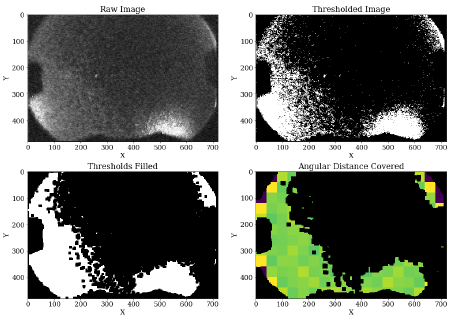
\includegraphics[width=10cm]{Cloud-Threshold.png}
    \caption{The above displays how an image captured by the D6 is manipulated to determine the cloudcover that would have existed when a fireball capture was made.}
    \label{Figure 8}
\end{figure}

\section{Flux!}
The last part of background to dig into is flux, or in other terms, the number of meteoroids or asteroids of a specific bolide energy that impact the Earth's atmosphere every year\cite{PBrown2002}.
This subject was touched on earlier when figure 2 was mentioned in relation to Peter Browns paper, and is central to determining if the D6 camera is performing to optimal standards.
To determine flux, there are two different equations given by Brown that we can use, the first being
\begin{equation}
    log(N) = a_0-b_0(log(E))
\end{equation}
and the second being
\begin{equation}
    log(N) = c_0-d_0(log(D)).
\end{equation}

Where $a_0=0.5677\pm0.015$, $b_0=0.90\pm0.03$, D is the asteroid/meteoroids width in meters, $c_0=1.568\pm0.03$, $d_0=2.70\pm0.08$, and N being the number of meteors with that specific energy.
It should also be noted that E can be determined using the optical energy $E_0$ with the equation\cite{PBrown2002}:
\begin{equation}
    E = 8.2508(E_0)^0.885
\end{equation}

With the energy and Number of meteors in hand, the goal would be to create a graph similar to Browns. And if successful, the graph created using data gathered by D6 should be roughly similar to that displayed in Brown's paper.
If not the case, then that indicated that work still needs to done to D6 to make it comparable to the other methods of detection discussed earlier.

